\documentclass[11pt,dvipsnames,svgnames]{report}

%PRÉAMBULE
\usepackage[french]{babel}
\usepackage[utf8]{inputenc}
\usepackage[table]{xcolor}
\usepackage[T1]{fontenc}
\usepackage[normalem]{ulem}
\usepackage{verbatim}
\usepackage{fancyhdr}
\usepackage{xcolor}
\usepackage{graphicx}
\usepackage{fancybox}
\usepackage{amsfonts}
\usepackage{amsmath}
\usepackage{ulem}
\usepackage{eurosym}
\usepackage{float}
\usepackage{adjustbox}
\usepackage{amssymb,amsmath,latexsym}
\usepackage{mathrsfs}
\usepackage[a4paper]{geometry}
\usepackage[bottom]{footmisc}
\usepackage{perpage}
\usepackage{multicol}
\PassOptionsToPackage{hyphens}{url}
\usepackage[breaklinks]{hyperref}
\usepackage[final]{pdfpages} 
\usepackage{appendix}
\usepackage{caption}
\usepackage{minitoc}
\usepackage{tikz}
\usepackage{setspace}
\usepackage{titlesec}
\usepackage{float}
\usepackage[section]{placeins}
\usepackage{rotating}
\usepackage{subfigure}
\usepackage{epsfig}
%\usepackage{mathpazo}
%\usepackage[scaled]{beramono}
\usepackage{menukeys}
\usepackage{etoolbox}
\makeatletter
\patchcmd{\ttlh@hang}{\parindent\z@}{\parindent\z@\leavevmode}{}{}
\patchcmd{\ttlh@hang}{\noindent}{}{}{}
\makeatother

\geometry{hmargin=2.5cm,vmargin=2cm}



\setcounter{secnumdepth}{4}
\setcounter{tocdepth}{4}


% En-têtes et pieds-de-page
\pagestyle{fancy}
\renewcommand\headrulewidth{1pt}
\fancyhead[L]{\small{\leftmark}}
\fancyhead[R]{
\includegraphics[scale=0.2]{images/logoasi.png}}
\fancyhfoffset{0pt}
\fancyfoot[R]{\setstretch{0,8}\small{GD, AH, MJ, RJ, AL}}
\fancyfoot[L]{
\includegraphics[scale=0.14]{images/LogoINSA.png}}
\renewcommand{\headrule}{{%
 \color{black}\hrule \headwidth \headrulewidth \vskip-\headrulewidth}}
\titleformat{\section}%
[hang]% style du titre (hang, display, runin, leftmargin, drop, wrap)
{\Large\bfseries}%changement de fonte commun au numéro et au titre
{\thesection}% spécification du numéro
{1em}% espace entre le numéro et le titre
{}% changement de fonte du titre


\begin{document}

\begin{titlepage}
\newcommand{\HRule}{\rule{\linewidth}{0.5mm}} 
\center 
\vspace*{\stretch{1}}\textsc{\huge Institut National des Sciences Appliquées de Rouen}\\[0.7cm] 
\LARGE Département ASI~\\[0.5cm]
\Large{Architecture des Systèmes d'Information} ~\\[1.5cm]
\textsc{\Large EC Informatique Répartie}\\[0.5cm] 

\HRule \\[0.4cm]
{ \huge \bfseries Document de Spécifications}\\[0.18cm] \HRule \\[1.5cm]
 
\LARGE \emph{\textbf{Projet}} \\
{Messagerie instantanée et visio/audio-conférence}\\[1.3cm]

\large
	\emph{\textbf{Auteurs}}\\
	Gautier \textsc{Darchen} \\ 
	Alexandre \textsc{Huat} \\ 
	Marie-Andrée \textsc{Jolibois} \\ 
	Romain \textsc{Judic} \\ 
	Alexandre \textsc{Le Lain}\\[0.3cm]
	
~\\[0.5cm]
\Large \emph{\textbf{Version}}\\
	\textsc{v0.00}

\vfill{\today} 

\begin{figure}

\includegraphics[width=4cm]{images/LogoINSA.png}\hfill

\includegraphics[width=3cm]{images/logoasi.png}
\end{figure}

%----------------------------------------------------------------------------------------

\vspace*{\stretch{1}} 
 \end{titlepage}

\newpage
\tableofcontents

\newpage


\chapter{Introduction}

L'application à développer est une plateforme de messagerie instantanée entre deux interlocuteurs. Elle permettra à ces interlocuteurs de communiquer tout en étant connectés sur des machines distantes. 


\section{Fonctions principales}
Les fonctions principales de cette application peuvent être scindées en trois catégories : 
\begin{itemize}
\item l'échange de messages ;
\item le filtrage des messages en fonction de leur contenu ;
\item l'utilisation d'un avatar.
\end{itemize}

Concernant la première fonctionnalité, les interlocuteurs pourront s'envoyer des messages écrits de façon instantanée. Ils auront en plus la possibilité de communiquer avec d'autres formats via un système de visio- ou audio-conférence intégré à l'application.

Le filtrage des messages prend en charge le contrôle parental et la modération. Les utilisateurs auront la possibilité de choisir d'activer ou non ce système de filtrage. De plus, ce dernier pourra être personnalisé.

Concernant la dernière fonctionnalité, un système d'avatar pourra être utilisé par les utilisateurs pour les conversations audio et écrites. Cette image n'est pas animée. 


\section{Utilisateurs}
Il existe plusieurs types d'utilisateurs dont les droits diffèrent.
\begin{description}
\item[Utilisateur \emph{lambda} :] il peut créer (ouvrir) une conversation, participer à une conversation qu'il sélectionne. Il peut paramétrer ses filtres. À la connexion, il choisit aussi un login et un avatar.
\item[Modérateur :] il peut émettre des messages de modération et supprimer des messages d'utilisateurs.
\end{description}
\vskip \baselineskip

\textcolor{red}{Plusieurs utilisateurs peuvent discuter en même temps sur une même conversation.}\\

Les seuls prérequis à l'utilisation sont l'installation et ouverture d'une application.

\chapter{Besoins détaillés}

\section{Spécifications fonctionnelles}

\textcolor{red}{L'IA est basique et à l'image d'un helpbot. L'IA est donc présente sur chaque conversation. L'utilisateur peut entrer des mots-clefs dans la conversation pour avoir des indications sur l'utilisation de l'application. }

~\\
\textcolor{red}{ Mots-clefs:
\begin{description}
\item[\og \textbackslash bonjour$\_$sophisme \fg\ :] répond à l'utilisateur \og Bonjour \texttt{<login>} \fg.
\item[\og \textbackslash help \fg\ :] affiche un menu d'aide avec l'ensemble des mots-clefs.
\item[\og \textbackslash help$\_$profil \fg\ :] indique à l'utilisateur comment paramétrer son profil.
\item[\og \textbackslash help$\_$filtre \fg\ :] indique à l'utilisateur comment paramétrer les filtres.
\item[\og \textbackslash help$\_$chat1 \fg\ :] indique à l'utilisateur comment ouvrir un salon de chat.
\item[\og \textbackslash help$\_$chat2 \fg\ :] indique à l'utilisateur comment rejoindre une conversation.
\item[\og \textbackslash help$\_$video \fg\ :] indique à l'utilisateur comment démarrer une conversation vidéo.
\item[\og \textbackslash help$\_$audio \fg\ :] indique à l'utilisateur comment démarrer une conversation audio.
\end{description}
}

~\\\\
\textcolor{red}{	Les utilisateurs ont des comptes temporaires qui n'existent que durant la durée de leur connexion au service. A l'ouverture de l'application ce dernier est redirigé vers la page \og Paramètres \fg\ où il précise différents champs le caractérisant (avatar, pseudonyme, mots à filtrer...).}
~\\\\
\textcolor{red}{Par défaut, lorsqu'un utilisateur démarre une conversation, il est seul avec l'IA jusqu'à l'arrivée d'autres utilisateurs.}

\subsection*{Cas d'utilisation}

Cette section présente les cas d'utilisation suivants :
\begin{itemize}
\item discuter ;
\item paramétrer le filtrage ;
\item filtrer les messages ;
\item se connecter.
\end{itemize}

\begin{figure}[H]
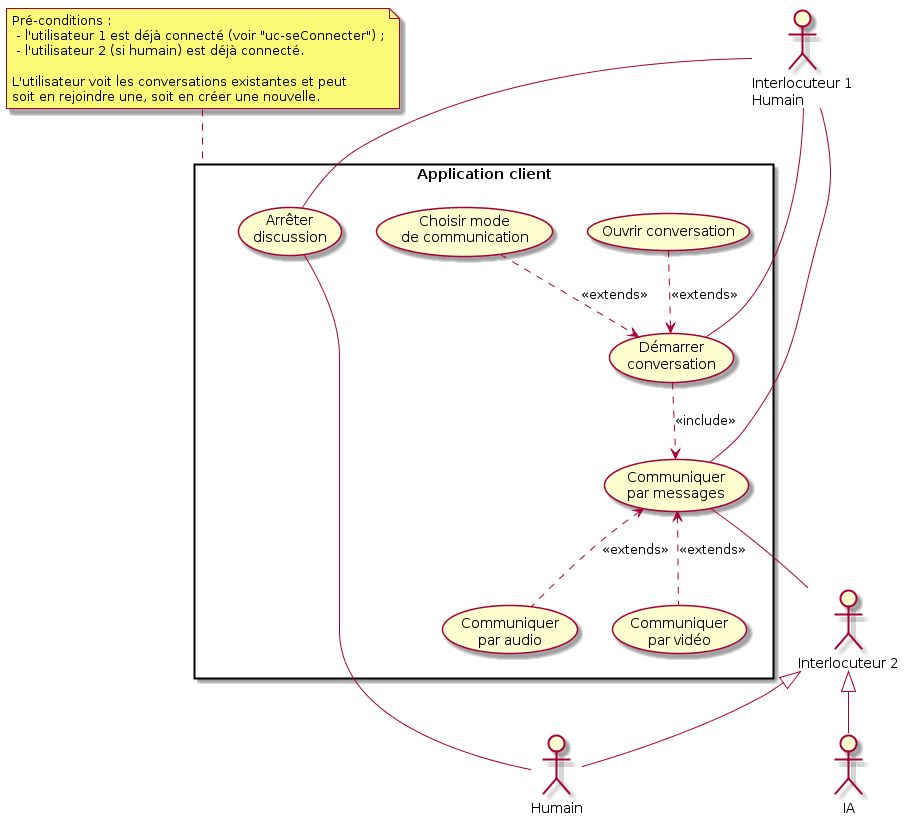
\includegraphics[scale=0.55]{images/uc-discuter.png}
\caption{Cas d'utilisation \textbf{discuter}}
\label{cas1}
\end{figure}
Le cas d'utilisation (figure \ref{cas1}) représente les interactions entre les différents interlocuteurs et les différents moyens mis à leur disposition pour communiquer.

\begin{center}
\begin{figure}[H]
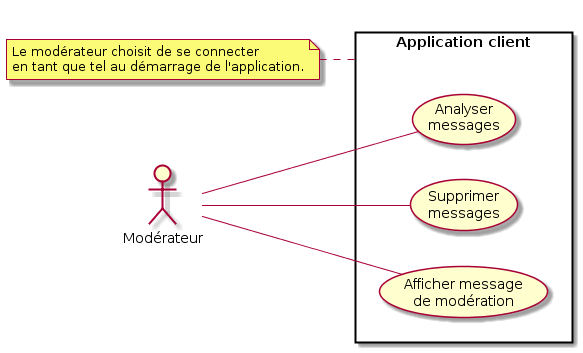
\includegraphics[scale=0.7]{images/uc-filtrerMessages.png}
\vspace{5\baselineskip}
\caption{Cas d'utilisation \textbf{filtrer les messages}}
\end{figure}

\begin{figure}
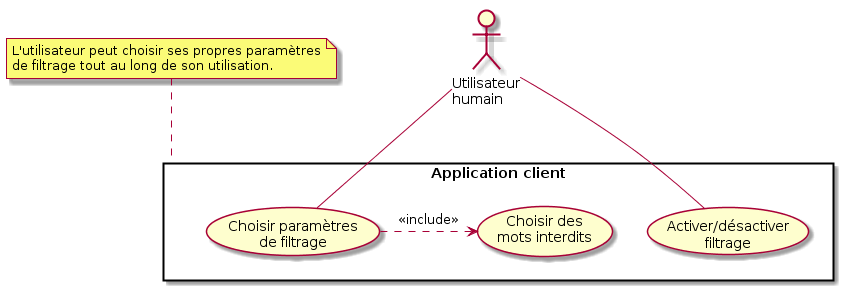
\includegraphics[scale=0.6]{images/uc-parametrerFiltrage.png}
\caption{Cas d'utilisation \textbf{paramétrer le filtrage}}
\end{figure}

\begin{figure}
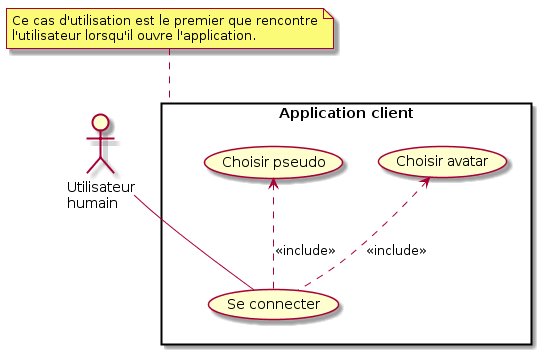
\includegraphics[scale=0.7]{images/uc-seConnecter.png}
\caption{Cas d'utilisation \textbf{se connecter}}
\end{figure}

\end{center}

\section{Spécifications d'interfaces}
\subsection*{Maquettes}

Cette section présente les maquettes de l'application.

\begin{figure}[H]
\centerline{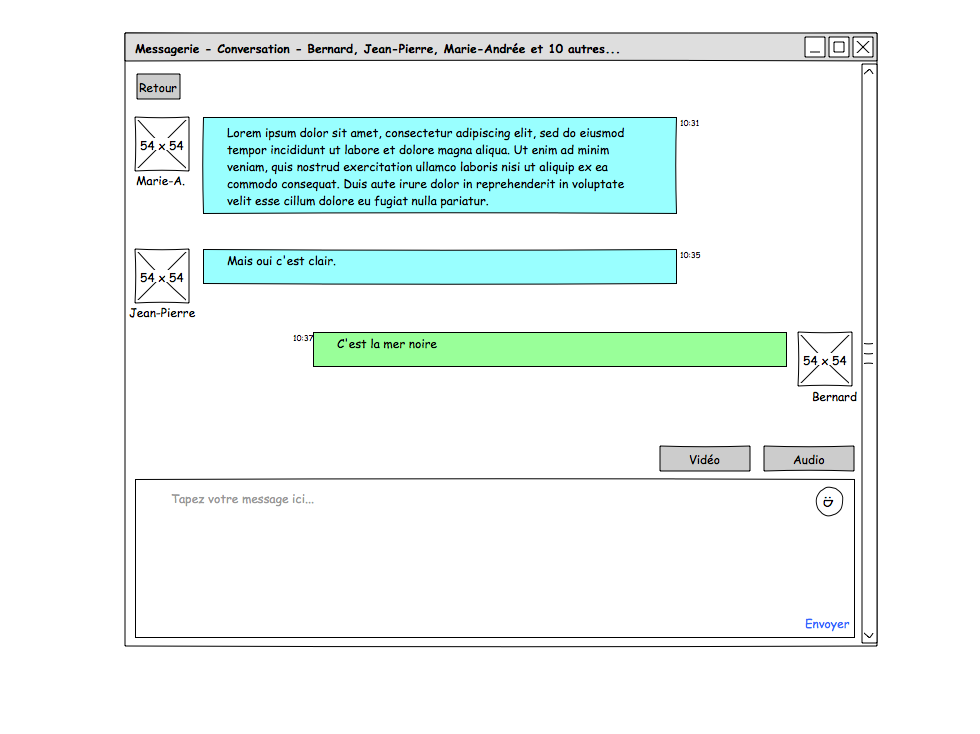
\includegraphics[width=0.95\textwidth]{maquette/maquette1.png}}
\caption{Un exemple de conversation texte}
\end{figure}

\begin{figure}[H]
\centerline{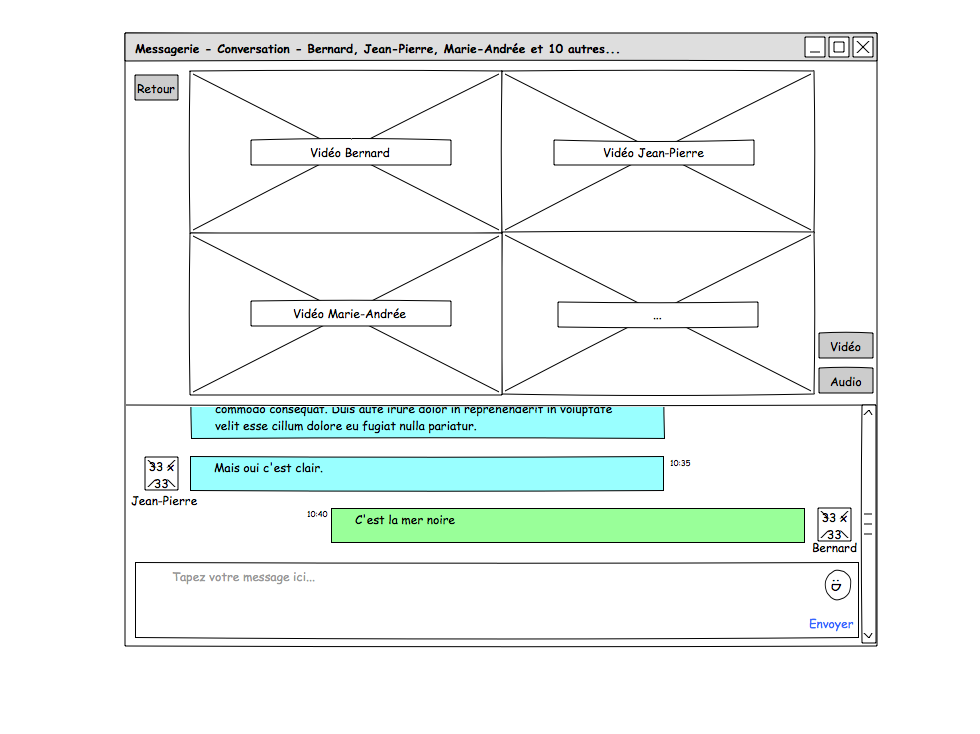
\includegraphics[width=0.9\textwidth]{maquette/maquette4.png}}
\caption{Conversation vidéo}
\end{figure}

\begin{figure}[H]
\centerline{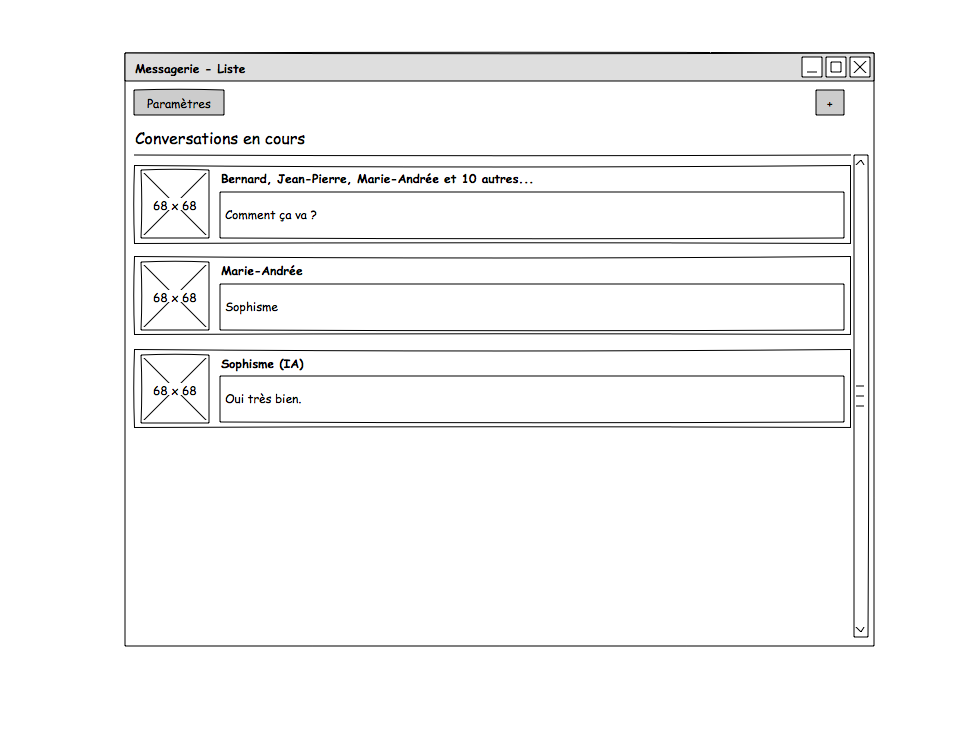
\includegraphics[width=0.9\textwidth]{maquette/maquette2.png}}
\caption{Liste des conversations}
\end{figure}

\begin{figure}[H]
\centerline{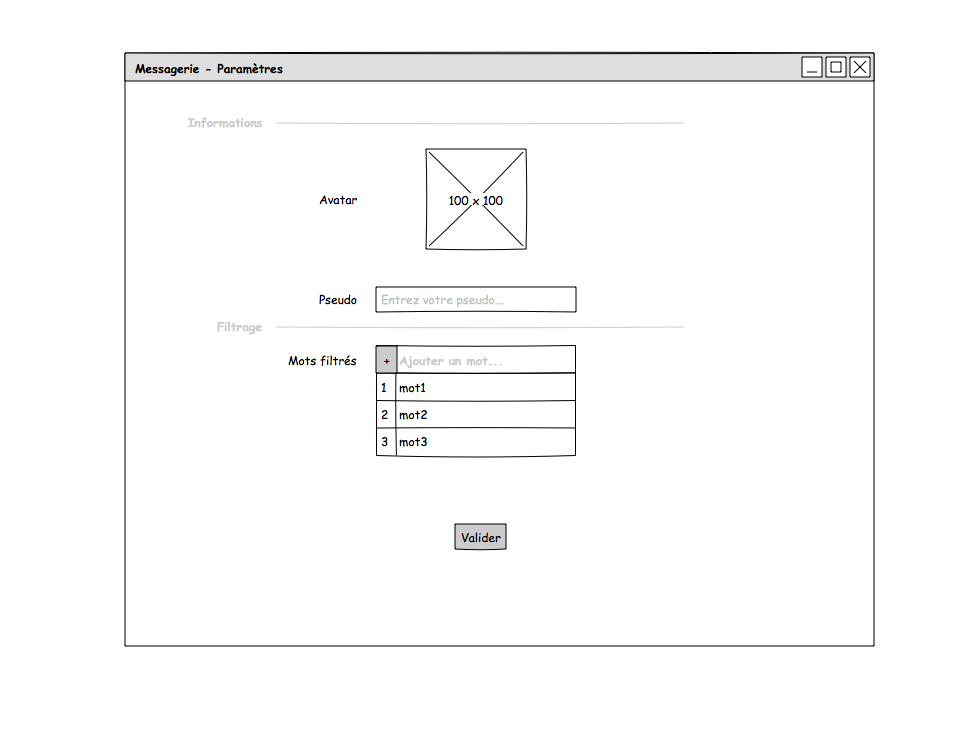
\includegraphics[width=0.9\textwidth]{maquette/maquette3.png}}
\caption{Interface des paramètres}
\end{figure}


\section{Spécifications opérationnelles}

Le système de messagerie répond instantanément.

De plus, les messages sont sauvegardés tant qu'il subsiste un utilisateur connecté à la conversation.

Le serveur qui héberge l'application est disponible à chaque instant $t$ pour permettre aux utilisateurs d'utiliser le service à n'importe quel moment.

\chapter{Contraintes}
\section{Contraintes matérielles}
L'utilisateur doit disposer d'une machine reliée à internet.

Pour profiter du service visio, l'utilisateur doit posséder un matériel de capture vidéo (webcam) et d'entrées/sorties audio.

Pour utiliser le service audio, l'utilisateur doit posséder une entrée et une sortie audio.

La majorité des calculs est réalisée côté serveur, ce qui n'implique pas un besoin de ressources conséquentes côté client.

\section{Contraintes logicielles}

Le client doit disposer du Java Runtime Environnement 8.

\end{document}